\section{Simulation results}
\begin{frame}
		\frametitle{Example of identifying $G_1(s)$ in Simulink }
	\begin{itemize}
			\item The simple power system presented was implemented in Simulink.
			\begin{figure}
					\includegraphics[width=0.8\textwidth]{./pictures/G0_sim.tikz}
			\end{figure}
	\end{itemize}
\end{frame}
\begin{frame}
		\frametitle{Can we find $S(s)$ without using a PMU}
	\begin{itemize}[<+->]
		\item To find $S(s)$ we need an estimate of $G_J(s)$.
\end{itemize}
				\begin{equation}
						G_J(s) = \frac{1}{2Hs+ K_d}
				\end{equation}
				\begin{equation}
						2H>>K_d
				\end{equation}
			\begin{equation}\label{eq:S_ident}
				S(s) \approx 2HsG_1(s)
			\end{equation}
		\includegraphics[width=0.8\textwidth]{./pictures/transf_comp.tikz}
\end{frame}
\begin{frame}
	\frametitle{Comparison of estimated sensitivity functions}
		\includegraphics[width=0.8\textwidth]{./pictures/S_sim.tikz}
\end{frame}
\begin{frame}
		\frametitle{Comparison of estimated $G_1(s)$}
		\includegraphics[width=0.8\textwidth]{./pictures/G0_req_sim.tikz}
\end{frame}

\section{Results from a real power plant}
\begin{frame}
	\frametitle{Dataset from Statkraft}
	\begin{itemize}[<+->]
		\item One of Norway's biggest power producers.
		\item They performed the tests from the draft requirements
		\item By chance I had PMU measurements from the same plant.
		\end{itemize}
		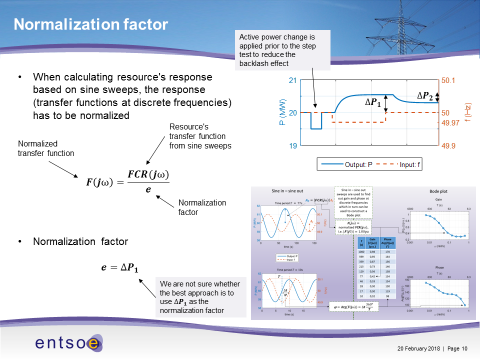
\includegraphics[width=0.8\textwidth]{./pictures/fcr.png}
\end{frame}
\begin{frame}
	\frametitle{Single line diagram of the plant}
	\begin{figure}
			\includegraphics{./pictures/plant_sld.tikz}
	\end{figure}
\end{frame}
\begin{frame}
	\frametitle{Datasets used}
	\begin{figure}
			\includegraphics[width=0.8\textwidth]{./pictures/signals.tikz}
	\end{figure}
\end{frame}
\begin{frame}
		\frametitle{Identified $G_1(s)$ using pmu signals}
	\begin{figure}
			\includegraphics[width=0.8\textwidth]{./pictures/lyon.tikz}
	\end{figure}
\end{frame}
\begin{frame}
	\frametitle{Estimated sensitivity functions}
		\begin{figure}[tb]
			\includegraphics[width=0.8\textwidth]{./pictures/S_pmu.tikz}
		\end{figure}
\end{frame}
\begin{frame}
	\frametitle{Estimated $G_1(s)$}
		\begin{figure}[tb]
			\includegraphics[width=0.8\textwidth]{./pictures/G0_pmu.tikz}
		\end{figure}
\end{frame}
